\documentclass[11pt]{article}
\usepackage[a4paper,margin=25mm]{geometry}
\usepackage{lmodern,amsmath,amssymb,amsthm,mathtools,microtype,booktabs,array,enumitem,xcolor,tikz,hyperref}
\usetikzlibrary{positioning,arrows.meta}
\hypersetup{colorlinks=true,linkcolor=blue!50!black,urlcolor=blue!50!black,citecolor=blue!50!black}
\definecolor{navy}{RGB}{31,53,79}
\newtheorem{theorem}{Theorem}[section]
\newtheorem{proposition}[theorem]{Proposition}
\newtheorem{remark}[theorem]{Remark}
\newtheorem{corollary}[theorem]{Corollary}
\newcommand{\cp}{\mathbb{CP}}
\newcommand{\R}{\mathbb R}
\newcommand{\Z}{\mathbb Z}
\newcommand{\cD}{\mathcal D}
\newcommand{\Om}{\Omega}
\newcommand{\Ext}{\operatorname{Ext}}
\title{\bfseries\color{navy} Finite Gain Graphs: A Verified Projective-Density Control, a Histories-Consistency Obstruction, and an Additive Holonomy Counterexample\\[4pt]
\large Director A, fourth grounding supplement}
\author{Kirtus Justus\\\small Research direction and scholarly responsibility\\\small Port Coquitlam, British Columbia, Canada\\[4pt]
\small AI-assisted mathematical review: ChatGPT (GPT-6), Director A}
\date{12 November 2026, B.C. Pacific Time}
\begin{document}
\maketitle
\begin{abstract}
We inspect directly the second-session papers G7 and G8 in the supplied Z2 edition and the B3/G3 packets. We give an explicit four-vertex \emph{simple} gain graph whose cyclic covering graph is primitive, thereby satisfying the walk-count growth premise of G8 Proposition 5.1 for every cyclic gain order. With a separately specified faithful complex character, the event rays are dense in $\cp^3$; the graph still fails the natural projective consistency requirement for a single histories decoherence functional across walk lengths. An exact cross-event witness rules out repair by scalar normalization. We also construct a gauge-invariant, nonnegative \emph{additive} holonomy-sensitive measure once terminal/root equality is available, precisely bounding G8's endpoint-blind no-go lemma. A sign slip in the \emph{proof} of G7's determinant identity is repaired without changing the identity. These are conditional mathematics and a source erratum, not a derivation of physical probability, dynamics, classical mechanics, or an ontology.
\end{abstract}
\noindent\textbf{Research status.} Initial External Grounding, G1 OPEN. No total ontology selected. All finite trial rows are retained in the machine-readable companion; reported computations are not independent scientific certification.

\section{Explicit carrier and primitive covering}
For $n\ge 2$ take the complete graph $K_4$ on vertices $0,1,2,3$, cyclic gain group $\Z_n$ (written additively), and gain $+1$ on $2\to3$, $-1$ on $3\to2$, and $0$ on all other oriented edges. This is a \emph{stipulated} abstract relation with no interpretation of arrows as physical time. The associated covering graph $\widetilde\Gamma_n$ has vertices $(v,g)$ and edges $(u,g)\sim(v,g+\varphi(u,v))$. All its vertices have degree three.

\begin{center}
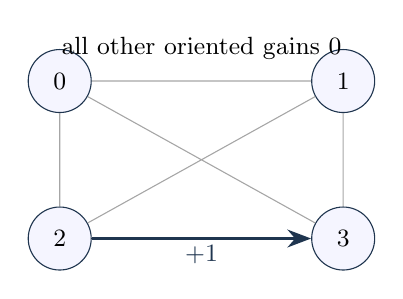
\begin{tikzpicture}[scale=1.0, every node/.style={font=\small}]
\node[circle,draw=navy,fill=blue!4,minimum size=8mm] (v0) at (-1.8,1) {$0$};
\node[circle,draw=navy,fill=blue!4,minimum size=8mm] (v1) at (1.8,1) {$1$};
\node[circle,draw=navy,fill=blue!4,minimum size=8mm] (v2) at (-1.8,-1) {$2$};
\node[circle,draw=navy,fill=blue!4,minimum size=8mm] (v3) at (1.8,-1) {$3$};
\draw[gray!70] (v0)--(v1) (v0)--(v2) (v0)--(v3) (v1)--(v2) (v1)--(v3);
\draw[navy,very thick,-{Stealth[length=3mm]}] (v2)--node[below,fill=white,inner sep=2pt] {$+1$} (v3);
\node at (0,1.42) {all other oriented gains $0$};
\end{tikzpicture}
\end{center}

\begin{theorem}[A concrete growth witness]\label{thm:growth}
For every integer $n\ge2$, $\widetilde\Gamma_n$ is connected and nonbipartite. Let $N_k(v,g)$ count $k$-edge walks beginning at $(0,0)$ and ending at $(v,g)$. Then for each fixed $v,g$,
\begin{equation}\label{eq:asymptotic}
N_k(v,g)=\frac{3^k}{4n}+O(\rho_n^k), \qquad 0\le\rho_n<3.
\end{equation}
In particular all $4n$ endpoint/gain counts tend to infinity \emph{simultaneously} along the entire integer sequence $k\to\infty$.
\end{theorem}
\begin{proof}
The path $0\to2\to3\to0$ has net gain $1$ and therefore its lifted repetitions reach every gain sector. Within a sector the lifts of paths whose net gain is $0$ connect all four base vertices, so the covering graph is connected. The base triangle $0\to1\to2\to0$, whose gains all vanish, lifts to an odd cycle. Hence the cover is nonbipartite. Its adjacency matrix $M_n$ is real symmetric, nonnegative, irreducible, aperiodic, and three-regular. Perron--Frobenius implies the eigenvalue $3$ is simple and strictly dominates every other eigenvalue in modulus. The associated unit eigenvector is the constant vector divided by $\sqrt{4n}$. The spectral decomposition of $M_n^k$ gives \eqref{eq:asymptotic} entrywise.
\end{proof}

\begin{corollary}[G8's dense-ray condition is realized explicitly]
For $n\ge3$, choose the faithful character $\chi(g)=e^{2\pi ig/n}$. For a walk event $S$, assign $v_S(y)=\sum_{w\in S,\;t(w)=y}\chi(\varphi(w))$.
The union over all walk lengths $k$ of the nonzero rays $[v_S]$ is dense in $\cp^3$ with its ordinary projective topology and transition-probability metric. This establishes an actual class of finite graph examples for the growth premise, \emph{not} the physical meaning of the metric.
\end{corollary}
\begin{proof}
By Theorem \ref{thm:growth}, for any finite prescribed nonnegative counts of walks with each endpoint and gain, there is one sufficiently large $k$ where the counts can all be selected as subsets of actual walks. Since $1+\chi(1)+\cdots+\chi(n-1)=0$, every negative contribution to a cyclotomic integer can be replaced by a finite sum of positive root-of-unity contributions. Thus every vector in $\Z[\chi(1)]^4$ occurs at some $k$. The ring contains $1$ and one nonreal number $\chi(1)$; integer combinations form a rank-two lattice when $n=3$ (and in any case its field of fractions $\mathbb Q(\chi(1))$ contains a dense rational plane in $\mathbb C$). Rays through such vectors are dense in $\cp^3$. These event vectors are a \emph{constructed} geometry, not identified preparations.
\end{proof}
\begin{remark}[Exact quantitative control]
For $n=3$, the $12\times12$ cover matrix first has all entries strictly positive at its fourth power. Starting from $(0,0)$, the minimum of the 12 gain/endpoint counts at $k=4,8,12$ is respectively $2,348,36126$; the totals are $3^k$. Every row for $k=0,\ldots,18$ is included without filtering.
\end{remark}

\section{An obstruction between successive walk lengths}
For $n=3$, put $\omega=e^{2\pi i/3}$. The represented adjacency operator, with columns indexed by sources, is the Hermitian matrix
\begin{equation}
A=\begin{pmatrix}
0&1&1&1\\1&0&1&1\\1&1&0&\bar\omega\\1&1&\omega&0
\end{pmatrix}.
\end{equation}
For an event of walks $S$ of length $k$ let $v_k(S)$ be the sum of its weighted endpoint vectors and $D_k(S,T)=\langle v_k(T),v_k(S)\rangle$. Let $\Ext S$ contain \emph{all} one-edge extensions of paths in $S$. Then
\(v_{k+1}(\Ext S)=A v_k(S).\)

\begin{proposition}[Failure of cylinder consistency]\label{prop:consistency}
The kernels $D_k$ cannot be made projectively consistent under $\Ext$ by multiplying each $D_k$ by an arbitrary nonzero scalar depending only on $k$. In particular, they do not define a normalized decoherence functional on cylinder events of infinite walks by that identification.
\end{proposition}
\begin{proof}
Let $S=\{0\to1\}$ and $T=\{0\to2\}$ at length one. Their endpoint vectors are $e_1,e_2$, hence $D_1(S,T)=0$. The vectors of their complete extensions are $Ae_1=(1,0,1,1)^T$ and $Ae_2=(1,1,0,\omega)^T$, giving
\begin{equation}
D_2(\Ext S,\Ext T)=\langle Ae_1,Ae_2\rangle=1+\omega=\tfrac{1+i\sqrt 3}{2}\ne0.
\end{equation}
No nonzero scalar normalization can turn the nonzero cross term into zero. Furthermore, for $\Omega_k$ the event of all $k$-walks,
\(\mu_0(\Omega_0)=1,\mu_1(\Omega_1)=3,\mu_2(\Omega_2)=15,\)
since $A^2e_0=(3,2,1+\bar\omega,1+\omega)^T$. Normalizing at each length by its total mass gives $\mu_1(S)/3=1/3$, but $\mu_2(\Ext S)/15=3/15=1/5$. Both diagonal and off-diagonal forms of consistency fail.
\end{proof}
\begin{remark}[Scope]
Projective cylinder consistency is an \emph{additional requirement} when interpreting successive $k$ as refinements of one history. G8 proves fixed-length strong positivity and a Hilbert-space quotient; it does not assert this cross-length requirement. Proposition \ref{prop:consistency} therefore identifies a missing dynamics/history bridge and does \emph{not} refute G8's fixed-$k$ results. One could add a unitary update, dilation, clock, or different event algebra, but each requires a separate construction and a warranted operational interpretation. The same $K_4$ graph supports the ordinary classical Markov cylinder probabilities $|S|/3^k$, illustrating nonselection: those classical probabilities \emph{are} consistent under $\Ext$ but ignore the gains.
\end{remark}

\section{Endpoint-aware first-order holonomy observables}
G8 Lemma 3.1 correctly states that if one universal function $F_1:G\to\R$ is applied to the \emph{gain alone} for every walk on every graph, switching invariance makes $F_1$ constant. Dropping the endpoint-blindness hypothesis changes the assertion.
\begin{proposition}[Positive, additive, gain-sensitive measure]\label{prop:additive}
For $G=\Z_3$ and root vertex $x$, define for every fixed-length event $S$
\begin{equation}
\nu(S)=\sum_{w\in S} \mathbf 1_{t(w)=x}\bigl(1+\Re\chi(\varphi(w))\bigr).
\end{equation}
Then $\nu$ is nonnegative, finite-additive, invariant under every vertex switching, and dependent on nontrivial closed-walk holonomy. Its diagonal intersection kernel $D^{\rm cl}(S,T)=\sum_{w\in S\cap T}\mathbf 1_{t(w)=x}(1+\Re\chi(\varphi(w)))$ is strongly positive. There is no second- or higher-order interference.
\end{proposition}
\begin{proof}
For $\Z_3$ the weight is $2$ when $\varphi(w)=0$ and $1/2$ when it is $1$ or $2$. Additivity follows from disjoint summation and strong positivity from the nonnegative diagonal Gram representation. Switching changes the gain of a walk from $x$ to $x$ by conjugation, which is trivial in $\Z_3$. In $K_4$, the closed three-step walks $0\to1\to2\to0$ and $0\to2\to3\to0$ have respective gains $0$ and $1$, hence weights $2$ and $1/2$. An additive measure has $I_r=0$ for every $r\ge2$.
\end{proof}
\noindent This does not contradict G8 Lemma 3.1, since $\mathbf1_{t(w)=x}$ is not a function of gain alone. It \emph{does} defeat an interpretation that switching invariance plus positivity, without endpoint-blindness, forces interference of order two before the transport becomes observable.

\section{Proof erratum for G7, without changing its determinant law}
Let $B=\prod_{j=0}^{k-1}\langle a_j\mid a_{j+1}\rangle$ with $a_k=a_0$ and $e^{i\theta}=B/|B|$. In the proof of G7 Proposition 4.3, consecutive horizontal phases obey
\(\alpha_{j+1}=\alpha_j-\arg\langle a_j\mid a_{j+1}\rangle.\)
Hence the \emph{terminal} lift is
\begin{equation}
\widetilde a_k=e^{-i\theta}a_0, \qquad U a_0=e^{-i\theta}a_0, \qquad T=e^{+i\theta}U\vert_{a_0^\perp}.
\end{equation}
The source proof instead writes a positive terminal exponent and negative tangent conversion. Those two signs must be reversed. Since $\det U=1$, we obtain
\begin{equation}
\det_{\mathbb C}T=e^{in\theta}\det(U\vert_{a_0^\perp})=e^{i(n+1)\theta}=(B/|B|)^{n+1}.
\end{equation}
\emph{The announced determinant law remains correct.} For a unit qubit triangle with $B=(9+3i)/16$, the horizontal lift ends at phase $(3-i)/\sqrt{10}$ and the tangent holonomy has eigenvalue $(4+3i)/5$, in accord with this correction.

\section{Reconciliation and ontology obligations}
\begin{center}
\small
\begin{tabular}{p{30mm}p{35mm}p{77mm}}
\toprule
Result & Status & Boundary / essential import \\
\midrule
$K_4$ cover counts & Proved, conditional data & Finite graph, assigned gains, graph covering, Perron--Frobenius \\
Dense $\cp^3$ rays & Proved in mathematical model & Faithful complex character, sum-of-walk-amplitudes map, ray equivalence \\
Cross-length $D_k$ & Obstruction proved & The \emph{natural} all-path extension; alternative history definitions not excluded \\
First-order $\nu$ & Proved countercontrol & Closed-walk endpoint information; falls outside G8 endpoint-blind lemma \\
G7 determinant & Theorem retained; proof patch & Source's horizontal-lift signs amended; no physical holonomy extracted \\
Operational measurement & Unresolved & Empirical preparation/readout, effects, frequency, calibration \\
Dynamics and time & Unresolved & Strongly consistent process, choice of update, clock, reversible evolution \\
Classical mechanics & Unresolved & Symplectic phase space, Hamiltonian flows and controlled limit \\
\bottomrule
\end{tabular}
\end{center}
The results are mathematical reductions, not a proof that any stipulated prephysical primitive exists in nature. The graph measure and a classical counting measure remain alternative completions of the same finite data. Director G3 independently supplies further nonselection controls for mixed-state tomography; Director B3 supplies conditional local-instrument selection boundaries. Neither closes these emergence obligations.

\section*{Methods, provenance and source context}
This supplement was generated from inspection of the \emph{actual} G7/G8 PDFs in the user-supplied Z2 archive and the B3/G3 submissions, rather than the disposition alone. Exact SymPy identities, finite-cover enumeration for $n=2,\ldots,8$, and every $k=0,\ldots,18$ count for $n=3$ appear in \texttt{verify\_A4\_independent.py} and its JSON. Direct B3 and G3 mathematical verifiers reran. G8's original program reran with its predicates passing; several floating-point entries differ in the last digits, so no byte-identical reproduction is asserted for those entries. Source baseline editions are left unchanged. The reviews and proofs remain AI-assisted and unrefereed, with no independent sub-agent or experimental measurement.

\smallskip\noindent\textbf{Primary literature used as scope checks, not as endorsement.}
F. Dowker, S. Johnston and R. Sorkin, \emph{Hilbert Spaces from Path Integrals}, J. Phys. A 43 (2010) 275302, \href{https://doi.org/10.1088/1751-8113/43/27/275302}{doi:10.1088/1751-8113/43/27/275302};
F. Dowker, S. Johnston and S. Surya, \emph{On Extending the Quantum Measure}, J. Phys. A 43 (2010) 505305, \href{https://doi.org/10.1088/1751-8113/43/50/505305}{doi:10.1088/1751-8113/43/50/505305};
T. Gelander, \emph{Limits of Finite Homogeneous Metric Spaces}, Enseign. Math. 59 (2013), 195--206, \href{https://doi.org/10.4171/LEM/59-1-8}{doi:10.4171/LEM/59-1-8};
H. Barnum, M. P. M\"uller and C. Ududec, \emph{Higher-order interference and single-system postulates characterizing quantum theory}, New J. Phys. 16 (2014) 123029, \href{https://doi.org/10.1088/1367-2630/16/12/123029}{doi:10.1088/1367-2630/16/12/123029}.
\end{document}
